\documentclass{article}
\usepackage{graphicx} % Required for inserting images
\usepackage{amsmath}
\usepackage{bm}
\usepackage{tikz}
\usetikzlibrary{bayesnet}
\usepackage{pgfplots}
\usepackage{textcomp}
\usepackage{enumitem}

\title{Dovetail}
\author{Patrick Sweeney}
\date{October 2023}

\begin{document}

\maketitle

\section{Decision theory}

Growth is a reinforcement learning problem, where the growth practitioner attempts to find optimal policies which maximise cumulative reward.






\section{Objective function}
The primary goal for most SaaS businesses is to maximize the present value of future revenue, often represented through the Customer Lifetime Value (CLV).

\begin{equation}
\arg\max PV(R) 
\end{equation}


\begin{equation}
\arg\max  \sum_{i=1}^{N} \text{CLV}_i 
\end{equation}

\begin{equation}
\arg\max  \sum_{i=1}^{N} \frac{MRR_i \times r_i}{1 + \text{WACC} - r_i}
\end{equation}



In this equation, the arguments are:
\begin{itemize}
  \item \( MRR_i \): Monthly Recurring Revenue for customer \(i\)
  \item \( r_i \): Retention probability for customer \(i\)
  \item \(\text{WACC}\): Weighted Average Cost of Capital
\item \( N \): Total number of customers
\end{itemize}

The our task is to set these arguments such that the output of the (objective) function is as high as possible.



\subsection{Generic objective function}

In the most general setting with multiple price metrics, the objective function is given by:

\begin{equation}
\arg\max \sum_{i=1}^{N} \left( \frac{\mathbf{P}_{i} \cdot \mathbf{V}_{i} \times r_i}{1 + \text{WACC} - r_i} \right)
\end{equation}

Here, the term \(\mathbf{P}_{i} \cdot \mathbf{V}_{i}\) represents the Monthly Recurring Revenue (MRR) for customer \(i\), broken down into price (\(\mathbf{P}_{i}\)) and volume (\(\mathbf{V}_{i}\)) vectors. The dimension of the price vector, \(\text{dim}(\mathbf{P}_{i})\), indicates the number of different pricing metrics applicable to customer \(i\). \\

\subsubsection{Example}
Consider a SaaS company that employs two pricing metrics: the number of seats and usage-based pricing (e.g., API calls). In this scenario, customer \(i\) might have the following vectors:

\[
\mathbf{P}_i = \begin{pmatrix}
    \text{Price per seat} \\
    \text{Price per API call}
\end{pmatrix}
=
\begin{pmatrix}
    10 \\
    0.05
\end{pmatrix}
\]

\[
\mathbf{V}_i = \begin{pmatrix}
    \text{Number of seats} \\
    \text{Number of API calls}
\end{pmatrix}
=
\begin{pmatrix}
    5 \\
    1000
\end{pmatrix}
\]

The Monthly Recurring Revenue (MRR) for this customer would be calculated as:

\[
MRR_i = \mathbf{P}_i \cdot \mathbf{V}_i = 10 \times 5 + 0.05 \times 1000 = 50 + 50 = 100
\]

Assuming a constant retention rate \( r_i = 0.95 \) and a monthly cost of capital \( \text{WACC} = 0.01 \), we can calculate the customer's CLV as:

\[
\text{CLV}_i = \frac{100 \times 0.95}{1 + 0.01 - 0.95} \approx 1583.33
\]


\subsection{Simple objective function}

In simpler cases, where each workspace \( i \) subscribes to a single package \( j \) with a fixed price, the objective function simplifies to:

\begin{equation}
\arg\max \sum_{i=1}^{N} \left( \frac{(P_j \times V_i) \times r_i}{1 + \text{WACC} - r_i} \right)
\end{equation}

Here, \( P_j \) is the fixed price per seat for the chosen package \( j \), and \( V_i \) is the number of seats specific to workspace \( i \). 

\subsubsection{Example}

In a SaaS company that offers \( j \) different packages, consider a scenario where each workspace \( i \) subscribes to one of these packages. In such a case, a  given workspace might have the following scalar values:

\[
P_j = 10 \quad (\text{Price per seat for package } j)
\]
\[
V_i = 5 \quad (\text{Number of seats for workspace } i)
\]

The Monthly Recurring Revenue (MRR) for this workspace would then be calculated as:

\[
MRR_i = P_j \times V_i = 10 \times 5 = 50
\]

Here, \( P_j \) is a fixed price determined by the chosen package \( j \), and \( V_i \) is the volume specific to workspace \( i \). \\

As before, we can assume a constant retention rate \( r_i = 0.95 \) and a monthly cost of capital \( \text{WACC} = 0.01 \). We can calculate the workspace's CLV as:

\[
\text{CLV}_i = \frac{50 \times 0.95}{1 + 0.01 - 0.95} \approx 791.67
\]


\subsection{Customer equity equation}

\section{Revenue drivers}


The presentation in section 1 it clear that the growth of a SaaS business is determined by a concise set of four fundamental variables:

\begin{itemize}
  \item \(\bm{N}\): Total number of customers
  \item \(\bm{P_j}\): Package price levels
  \item \(\bm{V_i}\): Seat volume
  \item \(\bm{r_i}\): Retention rate
\end{itemize}

These are the only variables that necessarily drive growth, and no others. \\ \\ \\ \\ \\ \\ \\ \\ \\ \\





\section{Product}

Product does not appear anywhere in the CLV equation. This is because there is no strict link between product and revenue growth.  \\

Put another way, the relationship between product and growth is \textbf{synthetic} and has to be empirically demonstrated, whereas the relationship between price/retention/volume and growth is \textbf{analytic} and follows directly from the math. \\
 
Put even more clearly, any revenue effect from product is \textbf{necessarily} mediated via the $N$, $P$, $V$ and $r$, variables, and the relationship between product and these variables is \textbf{probabilistic} at best and \textbf{nonexistent} at worst.  \\


\subsection{Product and growth}
While the causal link between product and price has been amply demonstrated, the link between product and acquisition, expansion, or retention is far more tenuous. \\

The following Bayesian network formalises the average average growth PM's beliefs:

\begin{center}
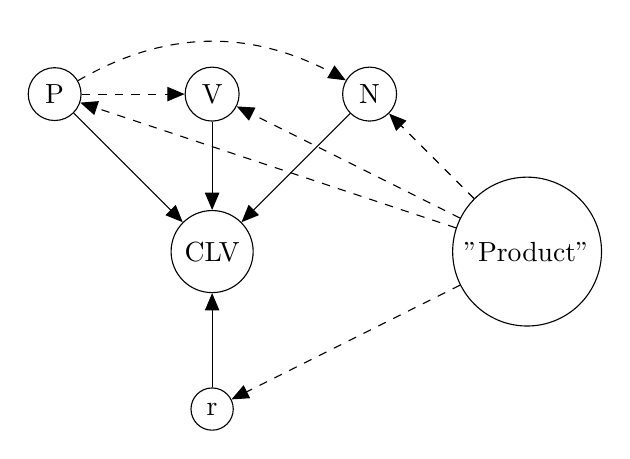
\begin{tikzpicture}
  % Define nodes
  \node[draw, circle] (CLV) at (2, 0) {CLV};
  \node[draw, circle] (P) at (0, 2) {P};
  \node[draw, circle] (V) at (2, 2) {V};
  \node[draw, circle] (N) at (4, 2) {N};
  \node[draw, circle] (r) at (2, -2) {r};
  \node[draw, circle] ("Product") at (6, 0) {"Product"};

  % Define edges with dotted lines
  \draw[->, dashed] (P) -- (V);
    \draw[->, dashed, bend left] (P) to (N);
  \draw[->, dashed] ("Product") -- (r);
  \draw[->, dashed] ("Product") -- (P);
  \draw[->, dashed] ("Product") -- (N);
  \draw[->, dashed] ("Product") -- (V);
  \draw[->] (P) -- (CLV);
  \draw[->] (V) -- (CLV);
  \draw[->] (N) -- (CLV);
  \draw[->] (r) -- (CLV);
\end{tikzpicture}
\end{center}


In the network above, standard arrows denote analytic statements (true by definition), and dashed arrows denote purported probabilistic causal links.  \\

It's worth noting that when PMs invoke the product\texttrademark , they typically mean product engagement. \\ \\ 

In do-calculus, one might say
\[
\begin{aligned}
& \mathbb{E}[V \mid \text{do}(P)] \\
& \mathbb{E}[N \mid \text{do}(P)] \\
& \mathbb{E}[P \mid \text{do}(\text{"Product"})] \\
& \mathbb{E}[V \mid \text{do}(\text{"Product"})] \\
& \mathbb{E}[N \mid \text{do}(\text{"Product"})] \\
& \mathbb{E}[r \mid \text{do}(\text{"Product"})] \\
\end{aligned}
\]

Or in plain English
\begin{itemize}
   \item The expected total customers and seat volume are conditionally dependent on interventions made on price
  \item The expected seat price, seat volume, total customers, and retention rate are conditionally dependent on interventions made on product engagement

\end{itemize}

The first claim is uncontroversial and follows from a statistical pattern so widespread it has been termed 'the law of demand'. The second claim requires requires evidence.

\subsection{Estimating casual networks}

Assuming that the expected seat price, seat volume, total customers, and retention rate are conditionally dependent on interventions made on product engagement, what would expect to see empirically? \\

Ideally, we would be able to check the proposed causal network against data and see if it holds. \\

There are three diferent types of network one might attempt to infer:

\begin{itemize}
   \item \textbf{Functional networks} use a measure of correlation between variables to infer connectivity. While this infers relationships between nodes with similar dynamics, it provides no explanation for how the relationship manifests.
  \item \textbf{Structural networks} seeks to reveal the directed (causal) connections in the system. Generally only possible via interventional (experimental) techniques but not directly from large observational multivariate time-series sets alone
\item  \textbf{Effective networks} are the middle ground, examining the directed (time-lagged) relationships between variables from their time-series, seeking to infer the “minimal neuronal circuit model” which can replicate and explain the time series of the nodes.
\end{itemize}

The key takeaway here is effective network inference is the gold standard for learning causal relationships from non-experimental data. \\

A natural measure for effective network inference is transfer entropy, as it measures the directed information flow between variables. \\

Put more rigorously, transfer entropy $T$ measures the amount of uncertainty reduced in predicting future values of a target variable $Y$, given the past values of itself and a source variable $X$. 
\[
T(X \rightarrow Y) = \sum p(y_{t+1}, y_t, x_t) \log \left( \frac{p(y_{t+1} \mid y_t, x_t)}{p(y_{t+1} \mid y_t)} \right)
\]

If there is a relationship between product and Y, then (equation)

If there is no relationship then conditoinally independent (equation)

We can safely say that if there is no transfer entropy between product engagement and expected seat price, seat volume, total customers, or retention rate, product engagement is irrelevant to growth. \\

Effective networks can be estimated at the level of the individual customer or entire company, using daily product usage data $f_i$ plus $P_i$, $V_i$, $N_i$ and $r_i$. Best-in-class algorithms utilise a greedy approach both capture synergies and eliminate redundancies in the network. Such algorithms can be implemented in Python using libraries like IDTxL.


\subsection{Modelling product engagement}

Assuming that there are conditional dependencies between product engagement and a real revenue growth driver, how should you analyse product engagement? \\



\subsubsection{Poisson processes}


We start by formalising a given customer's product usage behaviour as a Poisson process. \\

Poisson processes assume that in a time interval $dt$, individuals engage in a specific action with probability $\lambda dt$.  \\

Such a model predicts that the time-interval between two consecutive actions by the same individual $\tau$ —called the waiting of inter-event time—follows an exponential distribution.

$$p(\tau) = \lambda e^{-\lambda \tau}$$

It also follows that the the probability of observing $k$ events in an interval $t$ follows a Poisson distribution

\[
P(K = k; \lambda, t) = \frac{(\lambda t)^k e^{-\lambda t}}{k!}
\]

A key feature of the Poisson distribution is that the variance and mean are both given by the rate $\lambda$. Poisson distributions where the variance exceeds the mean are termed overdispersed. \\

In terms of underlying decision dynamics, Poisson product usage behaviour is the result of a First-Come-First-Serve (FCFS) decision rule, where feature usage operates on a "fair" basis—product engagement tasks in the order they arrive, and there's no priority or categorization that affects the order. 

STATISTICAL TESTS FOR POISSON
Pearson Chi2  divided by the degrees of freedom (dof) is greater than 1.0.

\subsubsection{Gamma poisson mixture (negative binomial process)}

The vast majority of product usage behaviour is overdispersed. The negative binomial process handles this by assuming that the rate parameter $\lambda$ of the Poisson process itself is a random variable, often following a Gamma distribution with parameters $\alpha$ and $\beta.$ \\

Under this model, the inter-event tau distribution $\tau$ follows a hypoexponential distribution, also known as the generalized Erlang distribution.

\[
p(\tau) = \alpha \beta e^{-\beta t} (1 - e^{-\alpha t})
\]

The tail of the distribution is still exponential, though 'fatter' than for a Poisson distribution. \\


Product count data then follows a negative binomial distribution.

\[
P(K = k; r, p) = \binom{k + r - 1}{k} (1-p)^{r} p^k
\]

This can be interpreted as the probability of observing $k$ events until you achieve $r$ successful events, given that the probability of an unsuccessful event is $p$.

STATISTICAL TESTS FOR NEGATIVE BINOMIAL


\subsubsection{Bursty process}

Bursty processes have an inter-arrival distribution $\tau$ that follows a power law distribution.

\[
P(\tau) \sim \tau^{-\alpha}
\]

The distribution of events is similarly fat tailed and is scale-free (independent of time).

\[
P(k) \sim k^{-\gamma}
\]


Burstiness score

\[
\text{Burst}(e, t) = \left( \frac{E_{t}}{E} - \frac{1}{T} \right)
\]


\[
B = \frac{\sigma - \mu}{\sigma + \mu}
\]


\subsubsection{Hidden Markov Model with Hierarchical Bayes}

Imagine you have mutipiple features and you want to model a latent engagement or customer satisfaction state. \\

Our observables are the product usage count data $\mathbf{Y} = \{Y_1, Y_2, ..., Y_k\}$ for $k$ features. \\

Starting with Bayes rule

\[
P(\boldsymbol{\theta} | \mathbf{Y}) = \frac{P(\mathbf{Y} | \boldsymbol{\theta}) \cdot P(\boldsymbol{\theta})}{P(\mathbf{Y})}
\] \\

Our goal is to estimate the parameter vector $\boldsymbol{\theta} = \{\boldsymbol{\pi}, \mathbf{A}, \mathbf{B}\}$ \\

$\boldsymbol{\pi}$ specifies the intial conditions in terms of the state distribution

\[
\boldsymbol{\pi}(i) = p(x_1 = i)
\]

$\mathbf{A}$ is a stochastic matrix specifying the jump probability from one hidden state to another

\[
\mathbf{A}(i,j) = p(x_t = j | x_{t-1} = i)
\]


$\mathbf{B}$ specifies the parameters of the 'class-conditional densities', which roughly speaking specify the component of the overall mixture distribution active as a function of hidden state $x$

\[
 p(y_t | x_t = j).
 \]

We start by setting priors

\[
P(\mathbf{A}) \sim \text{Dirichlet}(\alpha)
 \]

For possible state, we get a row in the hidden transition matrix. For example, if we are estimating a HMM with 4 states, we will have a 4x4 matrix, with four rows.

Each one of these $i$ rows will get its own Dirichlet distribution with concentration parameters $\boldsymbol{\alpha}_i = \{\alpha_{i1}, ..., \alpha_{ij}\}$




\]
\[
P(\lambda_i) \sim \text{Gamma}(k, \theta)
\]
\[
P(\mathbf{y}_t | s_t, \lambda) \sim \text{Multivariate Poisson}(\lambda[s_t])
\]
\[
P(s_t | s_{t-1}) = T[s_{t-1}, s_t]
\]
\[
P(\mathbf{Y}, s, T, \lambda, \alpha, k, \theta) = P(\mathbf{Y} | s, \lambda) \cdot P(s | T) \cdot P(T | \alpha) \cdot P(\lambda | k, \theta) \cdot P(\alpha) \cdot P(k, \theta)
\]






\subsection{Increasing product engagement}

\subsubsection{Poisson regression}

\subsubsection{Negative binomial regression}

\subsubsection{Poisson inverse Gaussian regression}








\section{Price}

\subsection{Consumer and producer surplus} 
Pricing is best formalised as a zero-sum game between the firm and the consumer. The total value \( V \) generated by a product for a consumer can be expressed as:

\[
V = R + CS
\]

Where \( V \) is the total value the product creates for the consumer, \( R \) is the revenue captured by the firm, and \( CS \) is the consumer surplus. \\

In turn, consumer surplus measures the consumer's net gain from the transaction, defined as the difference between the total value a consumer derives from a product  and the price they actually pay for it:

\[
CS = V - R
\]


It quickly becomes clear that the revenue optimal price is the price where consumer surplus is zero. With the possible exception of auctions, zero consumer surplus is an ideal scenario which is approached in practice but rarely reached. The key mechanism for achieving it will be price discrimination (sometimes euphemised as price differentiation). \\

\subsection{Demand curves and price response functions} 

The price response function specifies the volume demanded as a function of p

\[
V = f(p)
\]

There are many parametric flavours of price response function, but the most empirically realistic is the Gutenberg. 

\[
V = \beta_0 - \beta_1 p + \beta_2  \sinh (\beta_3(p_c - p))
\]

To bound volume between 0 and 1 and turn this into a survival function for the market's willingness to pay, we normalize
\[
S(p) = \frac{1}{Z} e^{\beta_0 - \beta_1 p + \beta_2  \sinh (\beta_3(p_c - p))}
\]
\[
\text{where } Z = \int e^{\beta_0 - \beta_1 p + \beta_2  \sinh (\beta_3(p_c - p))} \, dp
\]


The distribution of WTP becomes

\[
f(p) = \frac{\beta_1 + \beta_2 \beta_3 \cosh(\beta_3(p_c - p))}{Z} e^{-\beta_1 p - \beta_2 \sinh(\beta_3(p_c - p))}
\]
\[
\text{where } Z = \int e^{V(p)} \, dp
\]



To estimate this function from observed reservation prices, we use a Bayesian approach with priors

\begin{align*}
\beta_0 &\sim \text{Normal}(\mu_0, \sigma_0^2) \\
\beta_1 &\sim \text{Normal}(\mu_1, \sigma_1^2) \\
\beta_2 &\sim \text{Normal}(\mu_2, \sigma_2^2) \\
\beta_3 &\sim \text{Normal}(\mu_3, \sigma_3^2) \\
p_c &\sim \text{Exponential}(\lambda)
\end{align*}


\subsection{Price discrimination}

Let \( f(p) \) be the market-level price response function, denoting the volume \( v \) demanded at price \( p \). \\
The revenue function is:
\[
R(p) = p \times f(p)
\]

The inverse demand function, denoted as \( f^{-1}(v) \) or simply \( p(v) \), expresses price as a function of volume demanded. The revenue function in terms of \( v \) is:
\[
R(v) = v \times f^{-1}(v) \quad \text{or} \quad R(v) = v \times p(v)
\]

The revenue \( R \) generated by setting a price \( P \) can be expressed in integral form as:
\[
R(P) = \int_0^{f(P)} p(v) \, dx
\]

\subsubsection{No price discrimination}

Consumer Surplus \( CS \) is defined as the area between the inverse demand curve \( p(v) \) and the price level \( P \), up to the volue sold \( f(P) \). Mathematically, it is:

\[
CS = \int_0^{f(P)} (p(v) - P) \, dx
\]

Alternatively, it can be computed as the area under the inverse demand curve minus the revenue:

\[
CS = \int_0^{f(P)} p(v) \, dx - R
\]

We see here that for most demand curves, we are leaving a lot of money on the table, and this is bad.



\subsubsection{Some Price Discrimination (second and third degree)}

Instead of charging one price for everyone, we now chop the market into $i$ segments, each with its own demand curve $f_i(p_i)$ and price $P_i$. \\

The revenue becomes the sum of segment revenue
\[
R = \sum_i P_i \times f_i(p_i)
 \]

The (reduced) consumer surplus becomes

\[
CS = \sum_i \int_0^{f_i(P_i)} (p_i(v) - P_i) \, dv 
\]

and the additional revenue generated is 
\[
\Delta R = \sum_i P_i \times f_i(P_i) - P \times f(P) 
\]

This form of price discrimination is the most important, because it's the one encountered in practice. \\

The key techniques here will be discrimination based on product performance and volume.


\subsubsection{Perfect Price Discrimination (first degree)}
In the limiting case where $i \rightarrow \infty$, every customer becomes their own segment, and each is charged exactly their willingness to pay, capturing all the consumer surplus. \\

The revenue simplifies to

\[
R = \int_0^{f(P)} p(v) \, dv
\]

and

\[
CS = 0
\]


\subsubsection{Some Price Discrimination (second and third degree)}

\subsection{Multidimensional pricing}

Compared to one-dimensional pricing, multidimensional pricing can gen- erate significantly higher profits. The reason is that the profit potential, from a geometrical standpoint, resembles the area of a triangle. A one-dimensional or uniform price can only carve out a rectangle, whose area is necessarily smaller than the total area of the triangle. Unfortunately, multidimensional pricing is highly complex. Instead of one price decision, a company must make several. \\

The multidimensionality can derive from different price parameters. One can implement a volume-based price differentiation through a direct vol- ume discount, through the combination of fixed and variable price components, in the form of two- or multipart tariffs, or through discrete price points. In all cases it is critical to maintain effective fencing, i.e., to prevent a customer with a higher willingness to pay from buying at a lower price. This is the only way to come as close as possible to extracting the profit potential from the profit triangle. Ineffective fencing poses a significant risk. \\



\section{Value}

The price a customer is willing to pay, and thus the price the seller can achieve, is always a reflection of the customer’s perceived value of the product or service. If customers place a higher value on the product, then they are prepared to pay more. If the perceived value is lower than that of a competing product, they will only buy the product if the price is also lower (relative to the competitive product). But how does one rigorously define 'value'?


\subsection{Utility}

\begin{itemize}
    \item \textbf{Raw Part-Worth Feature Utility:} These are directly related to the \( \boldsymbol{\beta}_{i} \) values for each individual. Mathematically, you can consider them as samples from the conditional posterior distribution \( p(\boldsymbol{\beta}_i | \mathbf{X}, \mathbf{y}, \boldsymbol{\mu}, \boldsymbol{\Sigma}) \). Note that these will necessarily be Gaussian distributed because we've assumed a Gaussian prior. 
    
    \item \textbf{Normalized Part-Worth Feature Utility:} Often, these are the part-worth utilities normalized within each feature, typically so that they sum to zero for each feature. This is a transformation of the \( \boldsymbol{\beta}_{i} \) values. Mathematically, the normalized part-worth of level \( l \) of feature \( k \) is \( \beta_{ikl} - \text{mean}(\beta_{ik}) \).
    
    \item \textbf{Importance Scores:} These are typically calculated based on the range of part-worth utilities for each feature. They provide a measure of how impactful each feature is on the overall utility. Mathematically, the importance of feature \( k \) is \( \max(\beta_{ik}) - \min(\beta_{ik}) \).

     \item \textbf{Segments:} Bla bla bla

  \item \textbf{Feature correlations:} Bla bla bla
\end{itemize}


\subsubsection{Heterogeneity}
Different people value things and different levels.

\subsubsection{Complementarity, substitution, and correlations}

\subsection{Consumer choice theory} 

\subsubsection{Revealed preference}

\subsubsection{Budget constraint}

\subsubsection{Hicksian demand function}





Product usually has something to do with price. We will sidestep handwaving discussions about 'value' by  defining value as what people choose. \\

In economics, the standard approach is to modelling choice is to assume the following:
\begin{itemize}
  \item There is a finite set of $j$ MECE products among which the decision maker must choose.
  \item Products get chosen for a reason
  \item Each product can be described by a set of $k$ ordinal or categorical features
  \item There is a mathematical function $V$ that encodes the decision maker's preference for each product as a function of said features
  \item It's difficult to observe every relevant feature, so there is a utility function $U = V + \epsilon$ which takes into account both observed utility and random utility from unobserved features
  \item  Decision makers choose the product which maximises the utility function 
  \item  Only relative differences in utility matter and the scale of the utility is arbitrary
\end{itemize}

To bring price back into the equation, we will tack on the following assumptions
\begin{itemize}
  \item Price can be quantified as a categorical or ordinal feature of a product
  \item Price is utility reducing — $U(V, P = 0) $ \leq $U(V, P \geq 0)
  \item $U(V, P = 0) = U(P_r)$
  \end{itemize}

Kalish and Nelson (1988) show that a consumer's reservation price for a product is equal to the total utility contribution of the product divided by the marginal utility of money.
  





\subsection{Multinomial logit}

The first model you typically throw at this problem is the multinomial logit. A multinomial logit will tell you probability of class $j$ given a specific configuration of features $i$, assuming assuming Independence of Irrelevant Alternatives, homogeneity of preferences, linear additive utility, and no correlation across choices. \\

\[
P(j|i) = \frac{e^{z_{ij}}}{\sum_{j=1}^{J} e^{z_{ij}}}
\]

Here, $z_{ij}$ is the log-odds of choosing class $j$, representing some linear combination $i$ of the feature variables $\mathbf{x}$ weighted by their respective regression coefficients. 

\[
z_{ij} = \beta_0 + \beta_1 x_{1ij} + \beta_2 x_{2ij} + \ldots + \beta_k x_{kij} + \epsilon_{ij}
\]

Daniel McFadden won the Nobel Prize in Economics by taking this to the next logical step: defining $z$ as utility.

\[
U_{ij} = \beta_0 + \beta_1 x_{1ij} + \beta_2 x_{2ij} + \ldots + \beta_k x_{kij} + \epsilon_{ij}
\]


where a given $\beta_{ij}$ is called a part-worth utility and $\epsilon$ is Gumbel-distributed with parameters $\mu$ and $\beta$. \\

In this case, the probability of a product being chosen becomes

\[
P(j|i) = \frac{e^{U_{ij}}}{\sum_{j=1}^{J} e^{U_{ij}}}
\]

or in expanded form

\[
P(j|i) = \frac{e^{\beta_{0j} + \beta_{1j} \cdot x_1 + \beta_{2j} \cdot x_2 + \ldots + \beta_{kj} \cdot x_k}}{\sum_{j=1}^{J} e^{\beta_{0j} + \beta_{1j} \cdot x_1 + \beta_{2j} \cdot x_2 + \ldots + \beta_{kj} \cdot x_k}}
\]



To complement this, we can also introduce a social temperature term $T$

\[
P(j|i) = \frac{e^{U_{ij}/T}}{\sum_{j=1}^{J} e^{U_{ij}/T}}
\]

Expressing $T$ as an inverse temperature $1/\beta$ yields

\[
P(j|i) = \frac{e^{\beta U_{ij}}}{\sum_{j=1}^{J} e^{\beta U_{ij}}}
\]

We now recover the familiar quantal response function from McKelvey and Palfrey, where Inverse temperature $\beta$ paramterises the degree of bounded rationality. \\ \\

Given some data $\mathcal{D}$ including features \textbf{X} and observed choice behaviour \textbf{y}, we can estimate the parameters $\boldsymbol{\theta} = \{\beta_1, \beta_2, ..., \beta_k\}$ using maximum a posteriori. \\

Starting with Bayes rule

\[
p(\boldsymbol{\theta} | \textbf{X}, \textbf{y}) = \frac{p(\textbf{y} | \textbf{X}, \boldsymbol{\theta}
) \times p(\boldsymbol{\theta})}{p(\textbf{y} | \textbf{X})}
\]

Here, our posterior indicates that we're dealing with a discriminative model. As a result, the parameter vector $\boldsymbol{\theta}$ is jointly conditional on $\textbf{X}$ and $\textbf{y}$, rather than on $\mathcal{D}$ as a whole. \\

Similarly, the likelihood indicates that choices \( \textbf{y} \) are jointly conditional on \( \textbf{X} \) and \( \boldsymbol{\theta}\), unlike in the generative case where the likelihood often represents the joint distribution of both \( \textbf{X} \) and \( \textbf{y} \) given \( \boldsymbol{\theta} \), that is \( p( \mathcal{D}| \boldsymbol{\theta}) \) \\

Finally, the evidence follows the same pattern, replacing \( p(\mathcal{D}) \) with \( p(\textbf{y} | \textbf{X}) \). \\

Unlike in maximum likelihood where the goal is to maximise $\mathcal{L} = p(\textbf{y} | \textbf{X}, \boldsymbol{\theta})$, maximum a posteriori maximises the posterior, conditioned on the data. 

\[
\hat{\boldsymbol{\theta}}_{\text{MAP}} = \arg \max_{\boldsymbol{\theta}} p(\boldsymbol{\theta} | \mathbf{X}, \mathbf{y})
\]


The log posterior is equivalent to the sum of the log likelihood and the log prior.


\[
\log p(\boldsymbol{\theta} | \textbf{X}, \textbf{y}) = \log p(\textbf{y} | \textbf{X}, \boldsymbol{\theta}) + \log p(\boldsymbol{\theta})
\]

Because we only care about the MAP, which is unaffected by normalization by the evidence, we can say

\[
\hat{\boldsymbol{\theta}}_{\text{MAP}} = \arg \max_{\boldsymbol{\theta}} \log (p(\textbf{y} | \textbf{X}, \boldsymbol{\theta})) + \log (p(\boldsymbol{\theta}))
\]

Assuming a uniform prior, \( \log (p(\boldsymbol{\theta})) \) becomes a constant, such that

\[
\hat{\boldsymbol{\theta}}_{\text{MAP}} = \hat{\boldsymbol{\theta}}_{\text{MLE}} = \arg \max_{\boldsymbol{\theta}} \ln(p(\textbf{y} | \textbf{X}, \boldsymbol{\theta}))
\]


and the MAP estimate becomes the MLE estimate.

In this case, our model is 
\[
P(y|\textbf{X}) = \frac{e^{\beta_0 + \beta_1 X_1 + \beta_2 X_2 + \ldots + \beta_k X_k}}{\sum_{y'=1}^{J} e^{\beta_0 + \beta_1 X_1 + \beta_2 X_2 + \ldots + \beta_k X_k}}
\]

Our log likelihood function becomes
\[
\mathcal{L}(\boldsymbol{\theta}) = \sum_{n=1}^{N} \log \left( P(y_n|\textbf{X}_n) \right)
\]

and our optimization function becomes

\[
\hat{\boldsymbol{\theta}}_{\text{MLE}} = \arg \max_{\boldsymbol{\theta}} \mathcal{L}(\boldsymbol{\theta})
\]

The values of \( \hat{\boldsymbol{\theta}} = \{\beta_1, \beta_2, \ldots, \beta_k\} \) are the perceived utility of each product feature.


\subsection{Multinomial logit with hierarchical Bayes}

The assumptions of the standard multinomial choice model are quite restrictive. In particular, the homogeneous preference assumption leads to one utility function across the entire population, which is completely unrealistic. To account for heterogeneity and estimate individual utility functions for each potential customer, we bring in hierarchical Bayes. \\

Our choice model is identical as in the standard MNL case

\[
P_{ij} = \frac{e^{U_{ij}}}{\sum_{k \in J} e^{U_{ik}}}
\]


\[
U_{ij} = \mathbf{x}_{ij} \cdot \boldsymbol{\beta}_i
\]

We use Bayes rule

\[
p(\boldsymbol{\theta} | \mathbf{X}, \mathbf{y}) = \frac{p(\mathbf{y} | \mathbf{X}, \boldsymbol{\theta}) \times p(\boldsymbol{\theta})}{p(\mathbf{y} | \mathbf{X})}
\]

Our first step is setting a prior for our part-worth utilities $\beta_i$. An obvious choice is the multivariate Gaussian.

\[
p(\boldsymbol{\beta}_i) = \boldsymbol{\beta}_i \sim \mathcal{N}(\boldsymbol{\mu}, \boldsymbol{\Sigma})
\]

with hyperpriors 
\[
\boldsymbol{\mu} \sim \mathcal{N}(0, \mathbf{I})
\]

\[
\boldsymbol{\Sigma} \sim \text{Inverse-Wishart}
\]

At this point, it's worth explaining the 'hierarchy' in hierarchical Bayes. In this case, it consists of two levels. 

\begin{itemize}
\item The top level models the \textbf{heterogeneity in perceived part-worth utility across the population of potential customers}. Each individual will value different features differently, and this distribution is represented in the multivariate Gaussian joint posterior $p(\boldsymbol{\beta}_i | \mathbf{X}, \mathbf{y}, \boldsymbol{\mu}, \boldsymbol{\Sigma})$
  \item The bottom level models the \textbf{individual choice probabilities}. It takes a given customer's unique utility function from the top level, and models the probability of choice $j$ given a configuration of features.
\end{itemize}


Given that we're estimating a bunch of parameters, it's useful to write Bayes rule in explicit form to show exactly what's in the  parameter vector $\boldsymbol{\theta}$

\[
p(\boldsymbol{\beta}_i, \boldsymbol{\mu}, \boldsymbol{\Sigma} | \mathbf{X}, \mathbf{y}) = \frac{p(\mathbf{y} | \mathbf{X}, \boldsymbol{\beta}_i) \times p(\boldsymbol{\beta}_i | \boldsymbol{\mu}, \boldsymbol{\Sigma}) \times p(\boldsymbol{\mu}) \times p(\boldsymbol{\Sigma})}{p(\mathbf{y} | \mathbf{X})}
\]

where
\begin{itemize}
  \item \( p(\mathbf{y} | \mathbf{X}, \boldsymbol{\beta}_i) \) is the likelihood of the data given the individual-level parameters \( \boldsymbol{\beta}_i \).
  \item \( p(\boldsymbol{\beta}_i | \boldsymbol{\mu}, \boldsymbol{\Sigma}) \) is the prior on \( \boldsymbol{\beta}_i \) conditioned on the hyperparameters.
  \item \( p(\boldsymbol{\mu}) \) and \( p(\boldsymbol{\Sigma}) \) are the hyperpriors on \( \boldsymbol{\mu} \) and \( \boldsymbol{\Sigma} \).
  \item \( p(\mathbf{y} | \mathbf{X}) \) is the evidence 
\end{itemize}



The standard approach to estimating our parameter vector \( \boldsymbol{\theta} \) is to use Markov Chain Monte Carlo methods, specifically Gibbs sampling. Gibbs sampling iteratively samples each parameter from its conditional distribution while keeping all other parameters fixed, to approximate the joint posterior distribution. \\

As seen above, the posterior distribution we aim to approximate is:
\[
p(\boldsymbol{\theta} | \mathbf{X}, \mathbf{y}) = p(\boldsymbol{\beta}_i, \boldsymbol{\mu}, \boldsymbol{\Sigma} | \mathbf{X}, \mathbf{y})
\]

In Gibbs sampling, we do the following iteratively for each parameter in \( \boldsymbol{\theta} \):

\begin{enumerate}
    \item Sample \( \boldsymbol{\beta}_i \) from \( p(\boldsymbol{\beta}_i | \mathbf{X}, \mathbf{y}, \boldsymbol{\mu}, \boldsymbol{\Sigma}) \)
    \item Sample \( \boldsymbol{\mu} \) from \( p(\boldsymbol{\mu} | \boldsymbol{\beta}_i, \boldsymbol{\Sigma}) \)
    \item Sample \( \boldsymbol{\Sigma} \) from \( p(\boldsymbol{\Sigma} | \boldsymbol{\beta}_i, \boldsymbol{\mu}) \)
\end{enumerate}


This procedure can implemented quite easily in Python using libraries like PyStan or PYMC3. \\

Note: For most SaaS products, we're not dealing with features as such, but features with multiple discrete 'levels' which can be arbitrarily distributed among packages. An example could be rather than a feature called 'API calls', you may have three levels: 'API calls <100', 'API calls 100 - 1000' and 'API calls 1000+. 'In this case, it is customary to one-hot-encode each of the levels. After doing so, our part-worth utilities will denote levels $\boldsymbol{\beta}_{ikl}$ rather than features $\boldsymbol{\beta}_{ik}$. This in no way changes the estimation procedure, but simply the granularity of the features under consideration. \\


\subsection{MaxDiff}

MaxDiff (also known more correcty as best-worst scaling) infers the consumer's utility function by forcing them to make tradeoffs. \\

The likelihood $\mathcal{L}$ of observing the entire set of choices made by all respondents is usually the product of the individual choice probabilities. For a given respondent $r$ and a given set $S$, the choice probability $P_r(i,j|S)$ is

\[
P_r(i \text{ is best and } j \text{ is worst in } S) = \frac{e^{U_{ir} - U_{jr}}}{\sum_{m \in S} \sum_{n \in S} e^{U_{mr} - U_{nr}}}
\]

The likelihood function is therefore 

\[
\mathcal{L} = \prod_{r} \prod_{S \in \text{Sets}} P_r(i, j | S)
\]

The goal is to find the utility values $U_{ir}$ that maximize this likelihood function, or equivalently, that maximize the log-likelihood function:

\[
\log(\mathcal{L}) = \sum_{r} \sum_{S \in \text{Sets}} \log(P_r(i, j | S))
\]

Optimization algorithms like Newton-Raphson or gradient descent are typically used to find the utility values that maximize the log-likelihood. \\

These utilities are often scaled or averaged to produce a single utility value for each item, which can then be used for interpretation and decision-making.

\[
U_i' = U_i - \frac{\sum U_i}{\text{Number of Items}}
\]



\subsection{Van Westendorp}

\section{Bundling}
 The idea of packaging dates back to Chicago economist George Stigler. In the economics world, 'packaging' is called bundling —selling a bundle of features in a single package at one price.  \\

\subsection{A product is a group of bundles}

In the world of products, there is a hierarchy.

In set notation, the hierarchy can be represented as:




A product configuration \( C \) can be represented as a function \( C: X \rightarrow B \), where \( X \) is the set of all features and \( B \) is the set of all bundles. This function maps each feature \( x_k \) to a bundle \( b_j \). \\

Mathematically, \( C = \{ (x_1, b_{j1}), (x_2, b_{j2}), \ldots, (x_k, b_{jk}) \} \), where \( b_{jk} \) is the bundle to which feature \( x_k \) belongs. Every product configuration has the following properties: \\

\begin{itemize}
  \item \textbf{Uniqueness}: Each configuration \( C \) is unique and represents a specific arrangement of features into bundles.
  \item \textbf{Countable}: For \( k \) features and \( j \) bundles, there could be \( j^k \) possible product configurations, assuming each feature can belong to any bundle.
  \item \textbf{Order-Insensitive}: The order in which features are listed within a bundle does not affect the configuration, similar to how particles in a microstate are indistinguishable.
\end{itemize}

 
\subsection{Why bundle?}
 
 Packages/bundles are advantageous because unextracted willingness to pay from one feature to to another. This means that customer heterogeneity is reduced so that the price differentiation becomes more effective. \\

 In detail:

\begin{itemize}
\item Implicit price differentiation:  Customers may pay the same price for the bundle, but their willingness to pay for individual features varies. This creates a form of implicit price differentiation, allowing the company to capture more consumer surplus.
\item Higher price elasticity: When you bundle products with different elasticities, the overall elasticity of the bundle tends to be "averaged out" and reduced.
\item Information reduction: If only the bundled price is displayed, it's challenging for customers to deduce the price of individual components. When a price hike is wrapped up in a bundle, it may be less noticeable to consumers, mitigating negative reactions. Finally, In line with prospect theory, the pain of paying can be reduced when customers pay a single price for multiple items, as opposed to multiple individual prices.
\end{itemize}

 
\subsection{Types of bundling}

There are three types of bundle:
\begin{itemize}
\item No bundling. The features are offered and priced individually. The strength of unbundled sales is the ability to collect high prices from consumers with extreme tastes.
\item Pure bundling. Only the bundle is sold. The products cannot be bought individually. Pure bundling reduces effective buyer heterogeneity by aiming at aggregated reservation prices.
\item Mixed bundling. Here, both the bundle and the individual products are offered, i.e. a combination of separate pricing and pure bundling. Normally, prices are set for the individual products and the bundle.
\end{itemize}


Within mixed bundling and pure bundling, the price presentation can also go one of three ways

\begin{itemize}
\item Additive price bundling: The bundle price corresponds exactly to the sum of the prices for the individual products. We observe the use of additive price bundling on Amazon for books, kitchen, and household products.
\item Super-additive price bundling: The bundled price is higher than the sum of the individual prices. This form is rather rare. One example of its use is for complete collections of stamps, for which the seller can demand a premium for a complete set.
\item Sub-additive price bundling: The bundled price includes a discount, i.e., it is lower than the sum of the individual prices. This is the typical approach.
\end{itemize}





It is helpful to think of each feature $k$ as a continuous variable which can be used $x$ number of times by a given customer per month. In principal, every use of the feature provides value and it is reasonable to assume that the perceived utility of each use scales logarithmically in accordance with Gossen's principle.  \\

In this sense, all pricing begins as usage based pricing, until it is (optionally) quantized into discrete levels. 

This makes $X_k$ a random variable which has a distribution of monthly usage across the existing customer base.




Given $k$ features with $l$ possible levels, there are $l^k$ different possible product configurations. For a SaaS product with 10 features and three levels, that's about 60,000 potential packages. \\ \\ Assuming no knowledge of the consumer's utility function (not uncommon in SaaS), the maximum entropy distribution of product designs is uniform. This means that the probability of designing an optimal package, let alone three or four, is a rounding error. \\

A more rigorous approach is to configure the product to maximise an objective function, typically revenue, using integer, mixed-integer, or nonlinear programming.

\subsection{Package structure} 

There are well-known package structures, which differ in their constraints on the product configuration.
\begin{itemize}
\item All you can eat
\item Functional packages (use case packages)
\item Good / Better / Best
\item Platform plus functional packages
\item Build your own
\end{itemize}

In all of the following examples, we will consider \( k \) features \( x_1, x_2, \ldots, x_k \) which we need to turn into \( j \) bundles \( b_1, b_2, \ldots, b_j \). \\

Although the full product hierarchy looks like this

\[
\text{Level} \subset \text{Feature} \subset \text{Bundle} \subset \text{Product} \subset \text{Product Portfolio}
\]

we will only need to focus on bundles and features.

\subsubsection{All you can eat}

All you can eat offers is a single bundle of $k$ features. \\

By definition, there is only one product configuration available, therefore

\[
W = 1
\]


\subsubsection{Functional packages}

Functional packages are $j$ bundles with $k$ features, with no feature overlaps between bundles. \\

In combinatorics, this is the problem of partitioning a set into non-empty, disjoint subsets. We use Stirling numbers of the second kind to count the number of possible product configurations. 

\[
W = \frac{1}{j!} \sum_{i=0}^{j} (-1)^{j-i} \binom{j}{i} i^k
\]



\subsubsection{Good, Better, Best}

Good, Better, Best offers the same product at increasing quality levels, for instance \textit{Plus}, \textit{Pro}, and \textit{Enterprise}. \\

In this setup, each higher-level bundle \( j_{i+1} \) is a strict superset of the lower-level bundle \( j_i \). Features are distinguishable, but their order in the bundle is irrelevant. \\

In combinatorics, this problem is related to "Strictly Increasing Compositions of an Integer" or "Ordered Partitions with Non-Empty Subsets." The number of possible product configurations \( W \) is given by:
\[
W = \binom{k-1}{j-1}
\]


\subsubsection{Platform plus functional packages}

This model consists of a core platform and \( j \) functional packages, each with disjoint features. The platform includes \( m \) features, leaving \( k-m \) features to be distributed among the \( j \) functional packages.

\begin{itemize}
    \item \textit{Core Platform}: \( m \) features, with \( \binom{k}{m} \) ways to select them.
    \item \textit{Functional Packages}: \( j \) bundles, with \( k-m \) features distributed among them without overlap.
\end{itemize}

The total number of possible configurations \( W \) is given by:
\[
W = \binom{k}{m} \times \left( \frac{1}{j!} \sum_{i=0}^{j} (-1)^{j-i} \binom{j}{i} i^{(k-m)} \right)
\]


\subsubsection{Build your own}

In this case, the customer chooses one bundle, effectively setting \( j = 1 \). The complexity arises from the \( k \) features that can either be included or not in the selected bundle.

\begin{itemize}
    \item \textit{Feature Choices}: Each of the \( k \) features can be either included or excluded, resulting in \( 2^k \) possible configurations.
    \item \textit{Excluding Empty Bundle}: To avoid an empty package, one configuration is subtracted.
\end{itemize}

The total number of configurations \( W \) is therefore:
\[
W = 2^k - 1
\]

\subsection{Price metrics}

Compared to one-dimensional pricing, multidimensional pricing can gen- erate significantly higher profits. The reason is that the profit potential, from a geometrical standpoint, resembles the area of a triangle. A one-dimensional or uniform price can only carve out a rectangle, whose area is necessarily smaller than the total area of the triangle.

\subsection{Price models}

Price models 

\subsection{Optimization}

\textbf{Hanson and Martin model}

\[
\text{Maximize } Z = \sum_{b \in \text{Bundles}} p_b \cdot q_b - \sum_{i \in \text{Items}} c_i \cdot x_i
\]
\[
\text{Consumer Surplus}_j = V_{bj} - p_b
\]

\[
S = \{1, \ldots, n\} \quad k \in \{1, \ldots, n\} \quad i \in \{1, \ldots, L\} \quad j \in \{1, \ldots, m\}
\]
\[
R_{ji} = \text{Reservation price of customer segment } j \text{ for bundle } i
\]
\[
C_{ji} = \text{Cost of supplying one customer of segment } j \text{ with bundle } i
\]
\[
N_j = \text{Number of customers in segment } j
\]
\[
P_i = \text{Price assigned to bundle } i
\]
\[
e_{ji} = 
\begin{cases} 
1 & \text{if customer } j \text{ selects bundle } i \\
0 & \text{otherwise} 
\end{cases}
\]
\[
s_{ji} = \text{Consumer surplus of a customer in segment } j \text{ if that customer selects bundle } i
\]



\[
\text{WTP}_i = \frac{1}{|R_{\text{top20}}|} \sum_{r \in R_{\text{top20}}} \left( P_{\text{opt}, r} - P_{\text{avg}, r} \right)
\]






\section{Acquisition}

\subsection{New product diffusion}

\subsection{Value-based bidding}

Many ad platforms (e.g. Google, Meta) implement a technology called value-based bidding—an automated strategy that use “auction-time bidding”, in which the platform optimizes for conversion/conversion value in every auction you enter.


\subsection{Media mix modelling}

The typical approach to Media Mix Modelling is linear regression with some nonlinear transformations to account for shape and carryover effects.

\[
y_t = \alpha + \sum_{k=1}^{K} \beta_k f_k(g_k(x_{t,k})) + \gamma z_t + \epsilon_t
\]

\[
g_k(x_t) = x_t + \delta \cdot g_k(x_{t-1})
\]

\[
f_k(x) = \frac{x^{\eta}}{x^{\eta} + \theta^{\eta}}
\]



\begin{itemize}[label=$\bullet$]
  \item \( y_t \) is the revenue observable
  \item \( \alpha \) is baseline revenue
  \item \( x_{t,k} \) is the media spend on channel \( k \) at time \( t \)
  \item \( g_k \) is the adstock carryover transformation for media spend \( x_k \)
    \begin{itemize}[label=$\circ$]
      \item \( \delta \) controls the rate of effect decay
    \end{itemize}
  \item \( f_k \) is the shape transformation (Hill function) for media spend \( x_k \)
    \begin{itemize}[label=$\circ$]
      \item \( \eta \) is the steepness of the curve
      \item \( \theta \) is the channel's saturation point
    \end{itemize}
  \item \( \beta_k \) is the incremental revenue contribution of channel \( x_k \)
  \item \( \gamma \) is the incremental revenue contribution of covariate \( z_t \)
  \item \( z_t \) is another covariate (e.g., interest rates, S\&P, NASDAQ)
  \item \( \epsilon \) is Wiener noise
\end{itemize}

The \textbf{adstock carryover transformation} is an AR(1) model. This accounts for the fact that advertising has lagged effect which decay at a rate $\delta$.



The \textbf{shape transformation} is a Hill function, which models diminishing returns from ad saturation. Similar to the logistic function, the Hill function is S-shaped and implies that ad spending beyond some saturation threshold $\theta$ has no incremental effect. The ramp to saturation is controlled by the exponent $\eta$. \\


Taking a Bayesian approach to estimation

\[
\mathbf{p}(\boldsymbol{\theta} \,|\, \mathbf{y}, \mathbf{X}) \propto \mathbf{L}(\mathbf{y} \,|\, \mathbf{X}, \mathbf{Z}, \boldsymbol{\theta}) \cdot \mathbf{p}(\boldsymbol{\theta})
\]

\begin{itemize}
  \item \( \mathbf{p}(\boldsymbol{\theta} \,|\, \mathbf{y}, \mathbf{X}) \) is the posterior distribution of the parameters \( \boldsymbol{\theta} \) given the data \( \mathbf{y} \) and \( \mathbf{X} \).
  \item \( \mathbf{L}(\mathbf{y} \,|\, \mathbf{X}, \mathbf{Z}, \boldsymbol{\theta}) \) is the likelihood of the data \( \mathbf{y} \) given the predictors \( \mathbf{X} \), any additional covariates \( \mathbf{Z} \), and the parameters \( \boldsymbol{\theta} \).
  \item \( \mathbf{p}(\boldsymbol{\theta}) \) is the prior distribution of the parameters \( \boldsymbol{\theta} \).
\end{itemize}

We use MCMC to approximate the posterior with Gibbs sampling.

\subsubsection{ROAS}

ROAS is the change in revenue per dollar spent on advertising. It helps you understand the average return you're getting from an advertising channel.

In Bayesian terms, instead of a single value for each $\beta_k$, you would have a distribution of $\beta_k$ values. Therefore, the ROAS for each channel 
$k$ becomes a distribution:

\[
\text{ROAS}_{k} = \frac{\beta_k \,|\, \mathbf{p}(\boldsymbol{\theta} \,|\, \mathbf{y}, \mathbf{X}) \cdot f_k(g_k(x_{t,k}))}{x_{t,k}}
\]

The easy way to get channel ROAS it to set the spend for a particular medium (e.g., Google Ads, Facebook Ads) to zero for a selected time period. You then use the model to predict what the revenue would be if you hadn't spent any money on that medium. Because you also have the model's prediction of revenue with the actual spend for that medium, you can compare these two predictions: the revenue with zero spend and the revenue with actual spend. The difference between the two predicted revenues gives you the incremental revenue generated by that medium. You then divide this incremental revenue by the actual spend on that medium to get ROAS.

\subsubsection{Marginal ROAS}

Marginal ROAS (mROAS) measures the incremental effectiveness of additional spend on an advertising channel. It evaluates how much extra revenue you would get by spending one more unit of currency on that channel. mROAS is used for tactical allocation of incremental budget, helping you optimize your ad spend allocation by showing which channels give you the best incremental returns.


For channel $k$, you can compute the mROAS by considering a small change in the media spend $\delta x_{t,k}$ The mROAS can be formulated as:

\[
\text{mROAS}_{k} = \frac{\beta_k \,|\, \mathbf{p}(\boldsymbol{\theta} \,|\, \mathbf{y}, \mathbf{X}) \cdot \left[ f_k(g_k(x_{t,k} + \Delta x_{t,k})) - f_k(g_k(x_{t,k})) \right]}{\Delta x_{t,k}}
\]


\subsubsection{Acquisition curves}

The concept of marginal ROAS is closely related to the acquisition curve, also known as the "media efficiency curve" or "ad response curve." Both concepts help marketers understand how additional advertising spend impacts acquisition revenue.

In our context, the shape transformation (or Hill function) $f_k(x)$ serves as the acquisition curve for each channel. The overall acquisition curve is an average of these curves, each weighted by its contribution $\beta_k$ to revenue.

\[
\text{Acquisition curve} = \alpha + \sum_{k=1}^{K} \beta_k f_k(g_k(x_{t,k})) + \gamma z_t
\]

The Marginal ROAS would be the derivative of this overall acquisition curve with respect to the ad spend $x_{t,k}$ for a particular channel $k$

\[
\text{mROAS}_k = \frac{d}{dx_{t,k}} \left( \beta_k f_k(g_k(x_{t,k})) \right)
\]


\subsection{Activation}

'Activation' attempts to use product usage data in the first $t$ days of a customers' tenure to predict some economically relevant quantity of interest. For SaaS products, this is commonly during a free-trial or freemium period before the user has converted to becoming a full-blown paying customer. Implicitly, activation argues that interventions in this early period can influence volume, price, or retention. \\

An 'activation metric' is best conceived as the sole binary feature of a binary classifier. Because activation necessarily either happens or doesn't, its outcome is always $0$ or $1$. Similarly, because activation metrics were conceived to guide product teams (who hate complexity), the metric itself is always a coarse binary discretization of some continuous product usage behaviour. \\


A volume-based activation metric attempts to classify paid conversion.

\[
V = f(A)
\]


This paid conversion can be

\begin{itemize}
\item Generic: If paid conversion then 1 else 0
\item Seat threshold: If paid conversion $\geq k$ seats then 1 else 0
\end{itemize} 

A price-based activation metric attempts to classify land price at the level of the individual user.

\[
P = f(A)
\]

Dependent on the complexity of the price structure, this either means

\begin{itemize}
\item Package threshold: If price $\geq p_j$ then 1 else 0
\item Price threshold: If ARPU $\geq p_k$ then 1 else 0
\end{itemize}

The package threshold case corresponds to a simple structure with one price metric (seats) which differs according to choice of package $j$, whereas the price threshold approach considers the average revenue per user across all price metrics.



A retention-based activation metric attempts to classify retention rate.

\[
r = f(A)
\]

In practice, it's often simpler to classify customer lifetime $T$, which increases as $r$ increases.

\[
T = f(A)
\]

\begin{itemize}
\item Retention threshold: If lifetime $\geq T$ then 1 else 0
\end{itemize}

Note that retention-based metrics can quickly get dicey due to right censoring. To ensure a fair comparison, it's crucial to limit data to customers who both converted and had the opportunity to stick around for at least a year.

\subsubsection{Precision, Recall, F-score}

\subsubsection{Model comparison with net revenue function}

The net revenue or cost function is derived by apportioning a cost for every false positive and false negative and arriving at the overall revenue based on the correct and incorrect predictions.

\begin{itemize}
\item TP: 
\item FP:
\item TN:
\item FN: 
\end{itemize}

Jensen's inequality and the Jensen gap.



\section{Retention}

Retention is a key variable in the SaaS objective function. While there is no doubt that different customers have different retention rates, there is ongoing debate about whether these rates can be meaningfully moved once a given customer comes through the door. I will remain agnostic on this issue, and because this is ultimately a statistical question, I will show you how to answer it for the case of your particular SaaS business.




\subsubsection{Duration}

The survival time of a given customer is a random variable $T$.

We get a feeling for these times by expressing the random variable in different ways, each of which sheds light on the problem in a different way:

$$\prod_{i=0}^{T} r_i $$


\subsubsection{Hazard function}

The standard nonparametric approach to the survival function is to use a Nelson-Meier estimator.


\subsubsection{Survival function}

Retention is best formalised using a survival function. A survival function represnts the probability that a customer will survive past a certain time $t$, given that they have already survived up until $t$.

This survival function is also known as the complementary cumualtive distribution function of CCDF.

The standard nonparametric approach to the survival function is to use a Kaplan-Meier.


\subsubsection{Retention probabilities}

\subsubsection{Parametric survival analysis}

\subsubsection{Nonparametric survival analysis}

\subsubsection{Bayesian frailty models}

\subsubsection{Random survival forests}

\subsubsection{Projecting censored survival functions}

\subsubsection{Is retention probability fixed?}

\section{Expansion}

\section{Brand}

\subsection{Market definition}

\subsubsection{Principal components}

\subsubsection{Principal components}

\subsection{Category entry points}


\begin{itemize}
    \item \textit{Empty Bundles Allowed}: Some bundles can be empty, meaning they don't have to contain any features.
    \item \textit{Non-Strict Supersets}: A higher-level bundle \( j_{i+1} \) doesn't have to be a strict superset of a lower-level bundle \( j_i \). They could even have the same features, or \( j_{i+1} \) could have fewer features than \( j_i \).
    \item \textit{Independence of Bundles}: Each bundle can contain any subset of the \( k \) features, independent of what the other bundles contain.
\end{itemize}

In this relaxed scenario, each of the \( k \) features could go into any of the \( j \) bundles, giving \( j \) choices for each feature. Via a straightforward application of the product rule, the partition function is \\

\[
W = j^k 
\]

The problem with this scenario is the possibility of empty bundles, which is nonsensical. We need to subtract the number of configurations where one or more bundles are empty. Each bundle can be empty in \( (j-1)^k \) ways (since each feature now has \( j-1 \) choices). However, this would double-count cases where two bundles are empty, triple-count cases where three are empty, etc. Therefore, you would use the Principle of Inclusion-Exclusion to get the final count.

\[
W = j^k - \left[ \sum_{i=1}^{j} (-1)^{i+1} \binom{j}{i} (j-i)^k \right]
\]

However, we have a final problem. Not every feature has to get chosen. 
To account for the possibility that some features may not be chosen at all, we need to modify the counting formula. In the original formula \( W = j^k \), every feature has \( j \) bundle choices. When a feature can be left unchosen, it actually has \( j+1 \) choices: \( j \) bundles or not chosen at all. \\

So, the final formula that accounts for features that may not be chosen at all will be:
\[
W = (j + 1)^k - \left[ \sum_{i=1}^{j} (-1)^{i+1} \binom{j}{i} (j-i)^k \right]
\]

For the special case where we additionally constrain no overlap between the packages,

\end{document}
